\documentclass{beamer}

\usepackage[utf8]{inputenc}
\usepackage[spanish]{babel}
\usepackage{tikz}
\usepackage{booktabs}
\usepackage{pgfplots}
\usepackage{subfigure}
\usepackage{physics}
% \usepackage{titling} % adds \theauthor \thetitle etc
\usepgfplotslibrary{dateplot}

\newcommand{\titulo}{Python para el cálculo científico}
\newcommand{\autor}{Daniel Lubián Arenillas}
\newcommand{\fecha}{12 de febrero de 2018}
\newcommand{\git}{\texttt{git}}

\title{\titulo}
% \subtitle{¿Cómo usarlo?}
\author{\autor}
%\institute[IDR/UPM]{IDR/UPM}
\date{\fecha}
% \logo{
\includegraphics[height=1cm]{fig/git_logo.eps}}

\usepackage{listings}
\lstset{basicstyle=\ttfamily,numbers=left,numberstyle=\tiny}
\usepackage{verbatim}

% \usetheme{Rochester}
\usetheme{metropolis}
\metroset{block=fill, numbering=fraction, sectionpage=progressbar}%,subsectionpage=progressbar}%,titleformat=smallcaps}
% \usecolortheme{structure}

% \setbeamertemplate{frame footer}{\autor\,--\,\titulo}
\definecolor{azuletsiae}{RGB}{59,80,141}
\definecolor{azulclaroetsiae}{RGB}{197,208,228}
\definecolor{black1}{RGB}{26,28,34}
% \setbeamercolor{normal text}{fg=black1}
% \setbeamercolor{frametitle}{bg=azuletsiae}
% % \setbeamercolor{frametitle}{bg=black1}
% \setbeamercolor{progress bar}{fg=black1}
% \setbeamercolor{progress bar}{fg=azuletsiae,bg=white}
% \setbeamercolor{progress bar}{fg=azuletsiae,bg=azulclaroetsiae}
\titlegraphic{
	% 
\includegraphics[height=1cm]{fig/git_logo_name.eps}
	\hfill
	
\includegraphics[height=1.5cm]{fig/python.png}
}

% \usepackage{helvet}

% \usepackage[default]{lato}
% \renewcommand{\mddefault}{l}% switch default weight to light

\usepackage[sfdefault, light, lining]{FiraSans} %% option 'sfdefault' activates Fira Sans as the default text font
\usepackage[lining]{FiraMono}

%\usepackage[sfdefault,light]{roboto}

\usepackage[T1]{fontenc}


% \AtBeginSection[] % add toc at the beginning of a section, and highlight the next one
% {\begin{frame}
% 		\frametitle{Table of Contents}
% 		\tableofcontents[currentsection]
% \end{frame}}

 \addtobeamertemplate{frametitle}{}{%
 	\begin{tikzpicture}[remember picture,overlay]
 	\node[anchor=north east,yshift=1pt] at (current page.north east) {
\includegraphics[height=0.8cm]{fig/python.png}};
 	\end{tikzpicture}}

\begin{document}
	
\maketitle

\begin{frame}\frametitle{Hoy veremos}
	\tableofcontents
\end{frame}


\section{Presentando Python}

\begin{frame}\frametitle{Presentando Python}
	\begin{itemize}
		\item Creado por Guido van Rossum en 1991.
		\item Lenguaje de propósito general:
		\begin{itemize}
			\item Cálculo científico
			\item Desarrollo web
			\item Administración de sistemas
			\item GUIs
			\item Inteligencia artificial
			\item Todo es posible
		\end{itemize}
		\item Lenguaje multiparadigma, permite programación estructurada, orientada a objetos, funcional,...
		\item Lenguaje interpretado, no compilado.
	\end{itemize}
	
\end{frame}

\begin{frame}
	\centering
	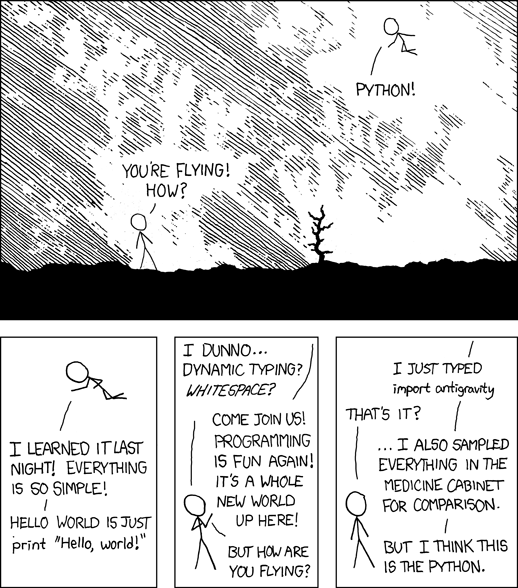
\includegraphics[height=8.5cm]{fig/xkcd.png}
\end{frame}

\begin{frame}\frametitle{Presentando Python}
	\begin{itemize}
		\item Dos versiones: 2.7 y \textbf{3.6}
		\item Libre, abierto y gratuito, con una comunidad enorme $\rightarrow$ todo a golpe de Google.
		\item Mil y una librerías abiertas y gratuitas.
		\item Rápido y fácil de escribir, puede ser lento de ejecutar.
	\end{itemize}

	Para escribirlo: Spyder, cuadernos Jupyter, Pycharm, VS Code, Atom, Geany, Notepad++...
\end{frame}

\subsection{Librerías importantes}

\begin{frame}\frametitle{Librerías importantes}
	\begin{figure}
		\subfigure{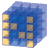
\includegraphics[height=1cm]{fig/numpy.png}}
		\subfigure{
\includegraphics[height=1cm]{fig/scipy.png}}
		\subfigure{
\includegraphics[height=1cm]{fig/matplotlib.png}}
		\subfigure{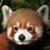
\includegraphics[height=1cm]{fig/pandas.jpg}}
		\subfigure{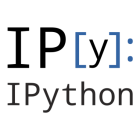
\includegraphics[height=1cm]{fig/ipython.png}}
	\end{figure}

	\centering
	\textbf{Numpy}: cálculo numérico

	\textbf{Scipy}: cálculo científico

	\textbf{Matplotlib}: graficado
	
	\textbf{Pandas}: análisis de datos
	
	\textbf{IPython}: consola interactiva
\end{frame}

\subsection{Programación orientada a objetos}

\begin{frame}\frametitle{Programación orientada a objetos}
	Un \textbf{objeto} tiene \textbf{métodos} (``funciones'') y \textbf{atributos} (``variables'') que lo constituyen.

	\begin{itemize}
		\item \texttt{A.shape}
		\item \texttt{z.conjugate()}
		\item \texttt{v.reshape((3,4))}
	\end{itemize}

	Todo Python trabaja con objetos\footnote{\tiny (hasta donde yo sé)}
\end{frame}


\section{Sintaxis básica de Python}

\begin{frame}\frametitle{Tipos}
	\centering
	\begin{tabular}{ccc}
		Entero 				& \texttt{integer} 			& \texttt{1} \\
		Con coma flotante	& \texttt{float} 			& \texttt{1.} \\
		Complejo 			& \texttt{complex} 			& \texttt{1. + 2j} \\
		Booleano 			& \texttt{boolean} 			& \texttt{True} \\
	\end{tabular}

	\begin{alertblock}{División de enteros}
		\lstinputlisting[language=Python]{code/int_div.py}
	\end{alertblock}
\end{frame}

\begin{frame}\frametitle{Contenedores}
	\textbf{Cadenas} $\rightarrow$ \texttt{s = "perro"} {\tiny inmutable}

	\textbf{Listas} $\rightarrow$ \texttt{l = [1, 'perro', True]}

	\textbf{Tuplas} $\rightarrow$ \texttt{t = (1, 'perro', True)} {\tiny inmutable}

	\textbf{Diccionarios} $\rightarrow$ \texttt{d = \{ 'O': 16, 'H2O': 18\}}

	\begin{alertblock}{Ojo: los índices van de \texttt{0} a \texttt{n-1}, como en C}
		\begin{itemize}
			\item \texttt{s[0]} devuelve \texttt{'p'}
			\item \texttt{l[-1]} devuelve \texttt{True}
			\item \texttt{t[3]} no existe
			\item \texttt{d['H2O']} devuelve \texttt{18}
			\item \texttt{l[0:2]} devuelve \texttt{[1, 'perro']} ($0 \leq i < 2$)
		\end{itemize}
	\end{alertblock}
\end{frame}

% \subsection{Sentencias de control}

\begin{frame}{Sentencias de control}
	\begin{block}{Condición: \texttt{if-elif-else}}
		\lstinputlisting[language=Python]{code/if.py}
	\end{block}
\end{frame}

\begin{frame}{Sentencias de control}
	\begin{block}{Bucle: \texttt{for}}
		\lstinputlisting[language=Python]{code/for.py}
	\end{block}
\end{frame}

\begin{frame}{Sentencias de control}
	\begin{block}{Bucle: \texttt{while}}
		\lstinputlisting[language=Python]{code/while.py}
	\end{block}
\end{frame}

\begin{frame}{Sentencias de control}
	\begin{block}{Iteración avanzada}
		\lstinputlisting[language=Python]{code/iter.py}
	\end{block}
\end{frame}

\begin{frame}{Sentencias de control}
	\begin{block}{\textsl{List comprehensions}}
		\lstinputlisting[language=Python]{code/list_comprehension.py}
	\end{block}
\end{frame}

\begin{frame}\frametitle{Funciones}
	\begin{block}{Definición}
		\lstinputlisting[language=Python]{code/function.py}
	\end{block}
	\begin{alertblock}{Paso por referencia}
		Los argumentos de las funciones se pasan por referencia, no por parámetro. Se mete la variable, no una copia, por lo que si se hace alguna modificación a \texttt{x} en el ámbito de la función, \texttt{x} cambiará fuera de la función.
	\end{alertblock}
\end{frame}

\begin{frame}\frametitle{Módulos}
	\begin{block}{Importar}
		\lstinputlisting[language=Python]{code/importar.py}
	\end{block}
\end{frame}

\section{Numpy: el \texttt{ndarray}}

\begin{frame}\frametitle{El \texttt{ndarray}}
	\begin{itemize}
		\item Es un clase eficiente para computación en \textsl{arrays}.
		\item Almacenan cualquier tipo, pero en todos los elementos el mismo.
		\item Atributos y métodos más útiles:
		\begin{itemize}
			\item \texttt{ndims}: entero con el número de dimensiones.
			\item \texttt{shape}: tupla con la forma.
			\item \texttt{reshape()}: cambia la forma según la tupla introducida.
			\item \texttt{T}: traspuesta
			\item \url{https://docs.scipy.org/doc/numpy/reference/generated/numpy.ndarray.html}
		\end{itemize}
	\end{itemize}
\end{frame}

\begin{frame}\frametitle{El \texttt{ndarray}}
	\begin{itemize}
		\item \texttt{np.array([1, 2, 3])}
		\item \texttt{np.zeros((2,))}
		\item \texttt{np.ones((2, 1))}
		\item \texttt{np.zeros\_like(a)}
		\item \texttt{np.empty((3, 4))}
		\item \texttt{np.linspace(0, 1, 6)}
	\end{itemize}
\end{frame}

\begin{frame}{Slicing}
	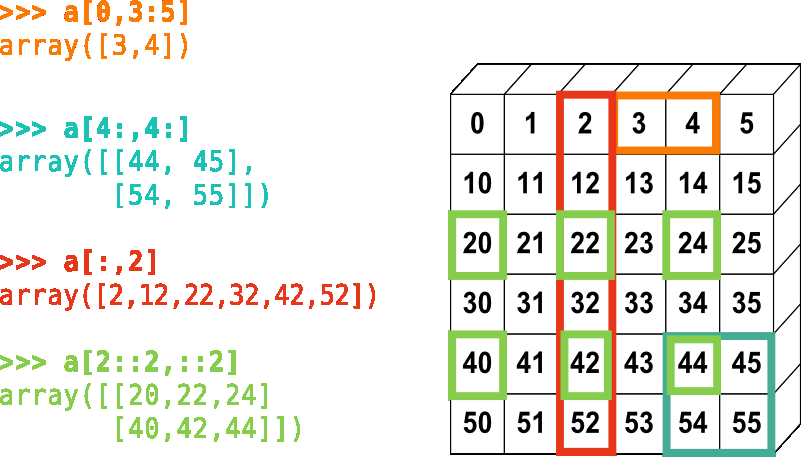
\includegraphics[width=\textwidth]{fig/slicing.png}
\end{frame}

\begin{frame}{Operaciones}
	\begin{itemize}
		\item \texttt{+}, \texttt{-}, \texttt{*}, \texttt{**}... funcionan \textsl{element-wise}
		\item El producto interno se puede hacer de varias maneras: \texttt{A.dot(B)}, \texttt{np.dot(A,B)}, \texttt{A @ B} (multiplicación de matrices de toda la vida)
	\end{itemize}
\end{frame}

\section{Scipy}

\begin{frame}{Submódulos útiles}
	\begin{columns}
		\begin{column}{0.5\textwidth}
			\begin{itemize}
				\item \texttt{scipy.linalg}\\ Álgebra lineal.
				\item \texttt{scipy.integrate}\\ Integración de integrales y EDOs.
				\item \texttt{scipy.optimize}\\ \textsl{solvers} para ecuaciones no lineales y optimizadores.
				\item \texttt{scipy.sparse}\\ Matrices dispersas.
				\item \texttt{scipy.constants}\\ Constantes.
			\end{itemize}
		\end{column}
		\begin{column}{0.5\textwidth}
			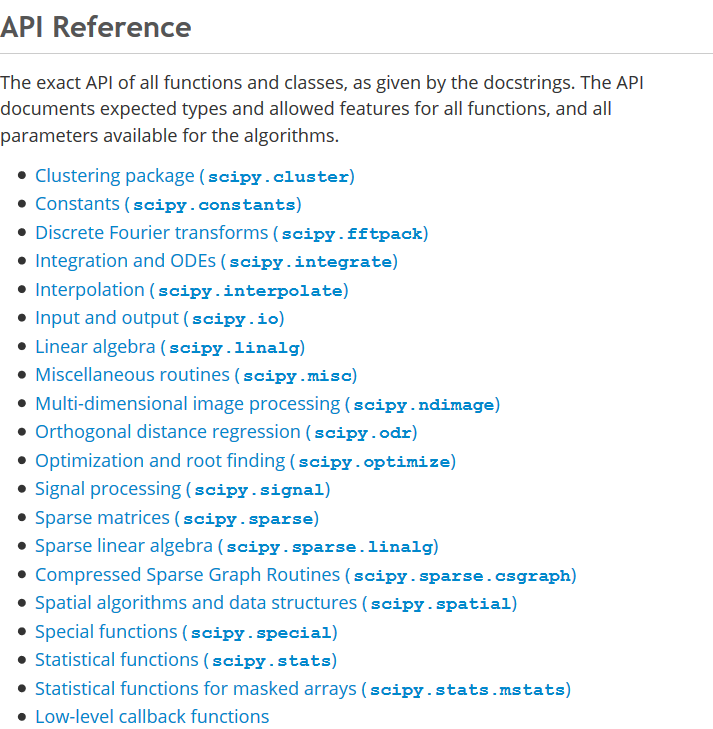
\includegraphics[width=\textwidth]{fig/scipy_api.png}
		\end{column}
	\end{columns}
\end{frame}

\begin{frame}\frametitle{\texttt{scipy.integrate}: integrales}
	
	\begin{block}{Integral de una función}

	$$ I = \int_0^{4.5} J_{2.5}(x)\dd{x}$$

		\lstinputlisting[language=Python]{code/quad.py}
	\end{block}
\end{frame}

\begin{frame}\frametitle{\texttt{scipy.integrate}: integrales}
	\begin{block}{Integral de una serie de datos}
		\lstinputlisting[language=Python]{code/trapz.py}
	\end{block}
\end{frame}

\begin{frame}\frametitle{\texttt{scipy.integrate}: EDOs}
	\begin{gather*}
		\dv[2]{w}{z} - z w(z) = 0\\
		w(0) = \frac{1}{\sqrt[3]{3^2}\;\cdot\; \Gamma\left(\frac{2}{3}\right)}\\
		\left.\dv{w}{z}\right|_{z=0} = - \frac{1}{\sqrt[3]{3}\;\cdot\; \Gamma\left(\frac{1}{3}\right)}\\
		\quad \\
		\text{Solución: } w(z) = \mathrm{Ai}(z)
	\end{gather*}
\end{frame}

\begin{frame}\frametitle{\texttt{scipy.integrate}: EDOs}
	\begin{gather*}
		\vb{y} = \begin{Bmatrix}
			w \\
			\dv{w}{z}
		\end{Bmatrix} \\
		\dv{}{z} 
		\begin{Bmatrix}
			y_0 \\ y_1
		\end{Bmatrix}
		= 
		\begin{bmatrix}
			0 & 1 \\
			z & 0 \\
		\end{bmatrix}  
		\begin{Bmatrix}
			y_0 \\ y_1
		\end{Bmatrix}
	\end{gather*}
\end{frame}

\begin{frame}\frametitle{\texttt{scipy.integrate}: EDOs}
	\begin{block}{Vamos a probarlo}
		\begin{itemize}
			\item Ir a uno de los repositorios de ese seminario:
			\begin{itemize}
				\item \url{https://gitlab.com/muse-dlubian/seminario_vida_moderna}
				\item \url{https://github.com/danbul/seminario_vida_moderna}
			\end{itemize}
			\item Descargar el cuaderno Jupyter: \texttt{python/ode.ipynb}
			\item Subirlo a \url{https://try.jupyter.org/}
		\end{itemize}
	\end{block}
\end{frame}

\begin{frame}\frametitle{\texttt{scipy.optimize}: \textsl{solvers}}
	$$
		\varepsilon = \frac{\Gamma(\gamma)}{ P^{\frac{1}{\gamma}} \sqrt{\frac{2\gamma}{\gamma -1}\left( 1 - P^{\frac{\gamma - 1}{\gamma}} \right)} }
	$$
	
	\begin{block}{Algunas posibilidades}
		\begin{itemize}
			\item Funciones escalares
			\begin{itemize}
				\item \texttt{brentq}: método de Brent
				\item \texttt{newton}: Newton-Raphson
			\end{itemize}
			\item Multidimensional
			\begin{itemize}
				\item \texttt{root}
				\item \texttt{fsolve}
				\item \texttt{broyden1}
			\end{itemize}
		\end{itemize}
	\end{block}

\end{frame}


% \section{Matplotlib.pyplot}

\end{document}
